\subsection{User actions requirements}
\subsubsection{Requirements 1}
List all locations in a table as
(a) links to single locations and
(b) allow sorting the table with
location names, distances, and the number of events at venue.
\begin{figure}[!h]
    \centering
    \begin{subfigure}{.45\textwidth}
        \centering
        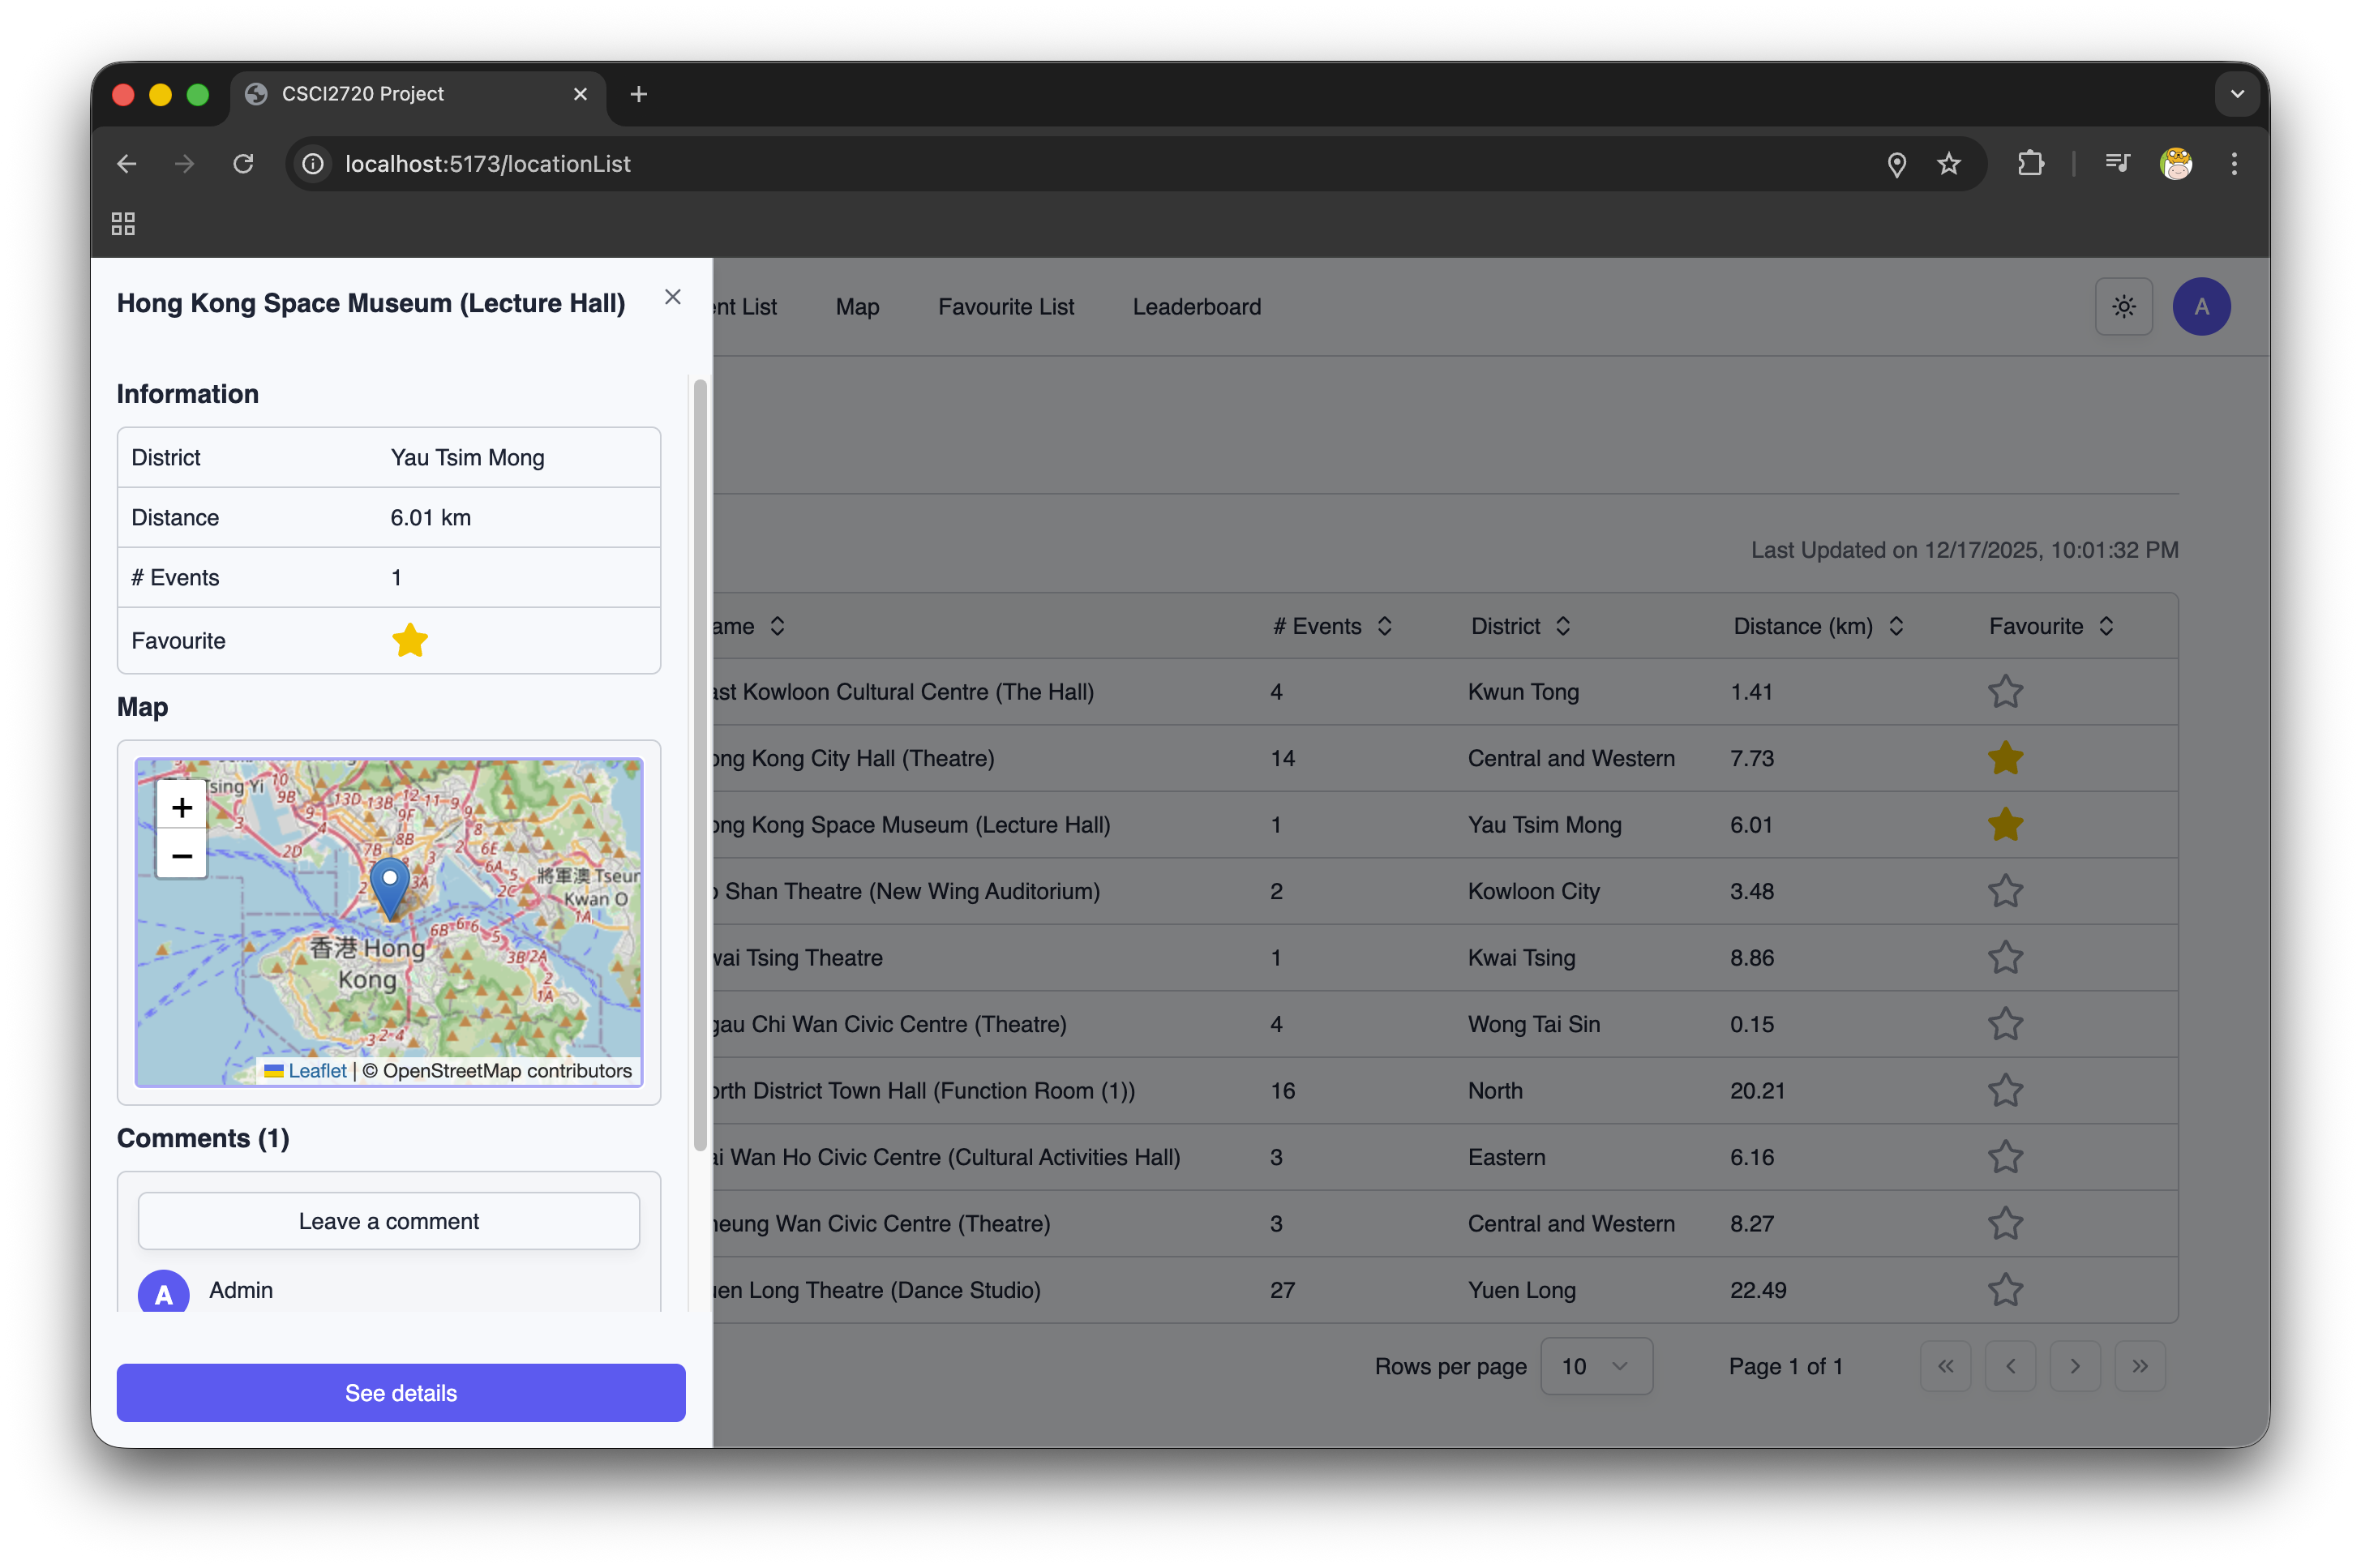
\includegraphics[width=\textwidth]{figures/req1a.png}
        \caption{Click on a row to check their details.}
        \label{subfig:req1a}
    \end{subfigure}
    \begin{subfigure}{.45\textwidth}
        \centering
        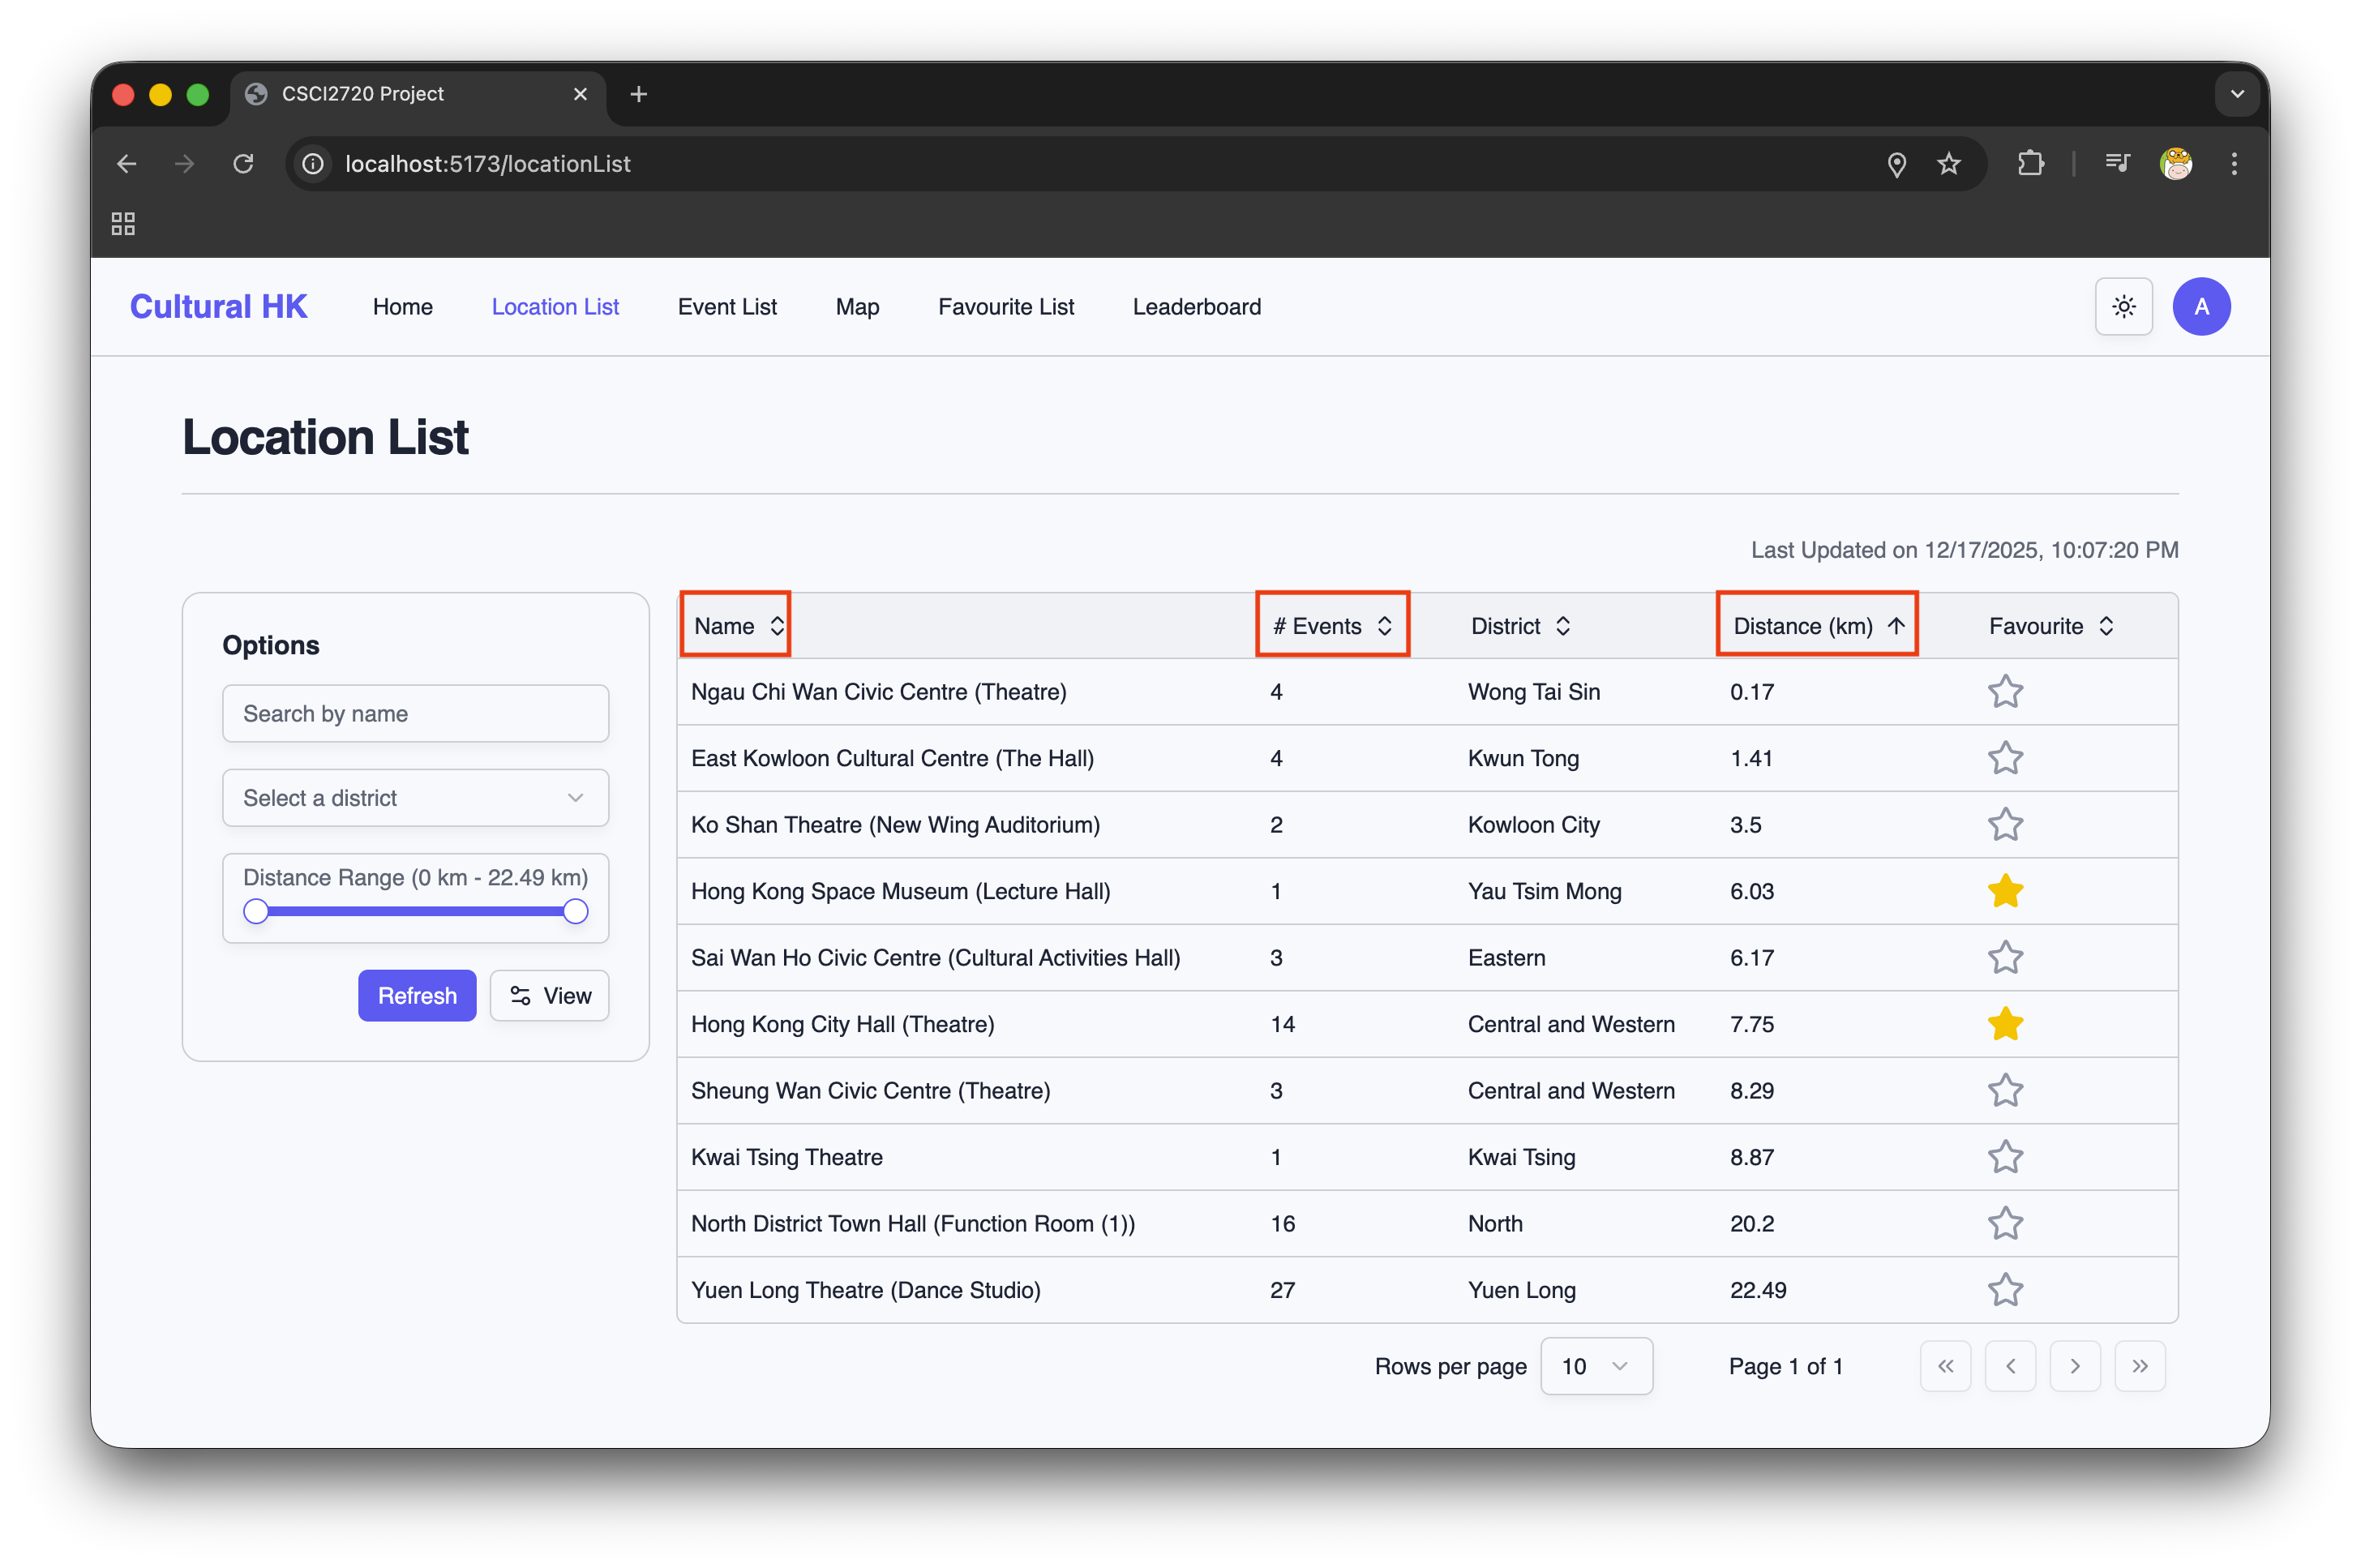
\includegraphics[width=\textwidth]{figures/req1b.png}
        \caption{
            Simply click on the column header to enable sorting.
        }
        \label{subfig:req1b}
    \end{subfigure}
    \caption{Location List with all the locations}
    \label{fig:location_list}
\end{figure}

\newpage
\subsubsection{Requirement 2}
(a) Show all locations in a map,
(b) with links to each single location.
\begin{figure}[!h]
    \centering
    \begin{subfigure}{.45\textwidth}
        \centering
        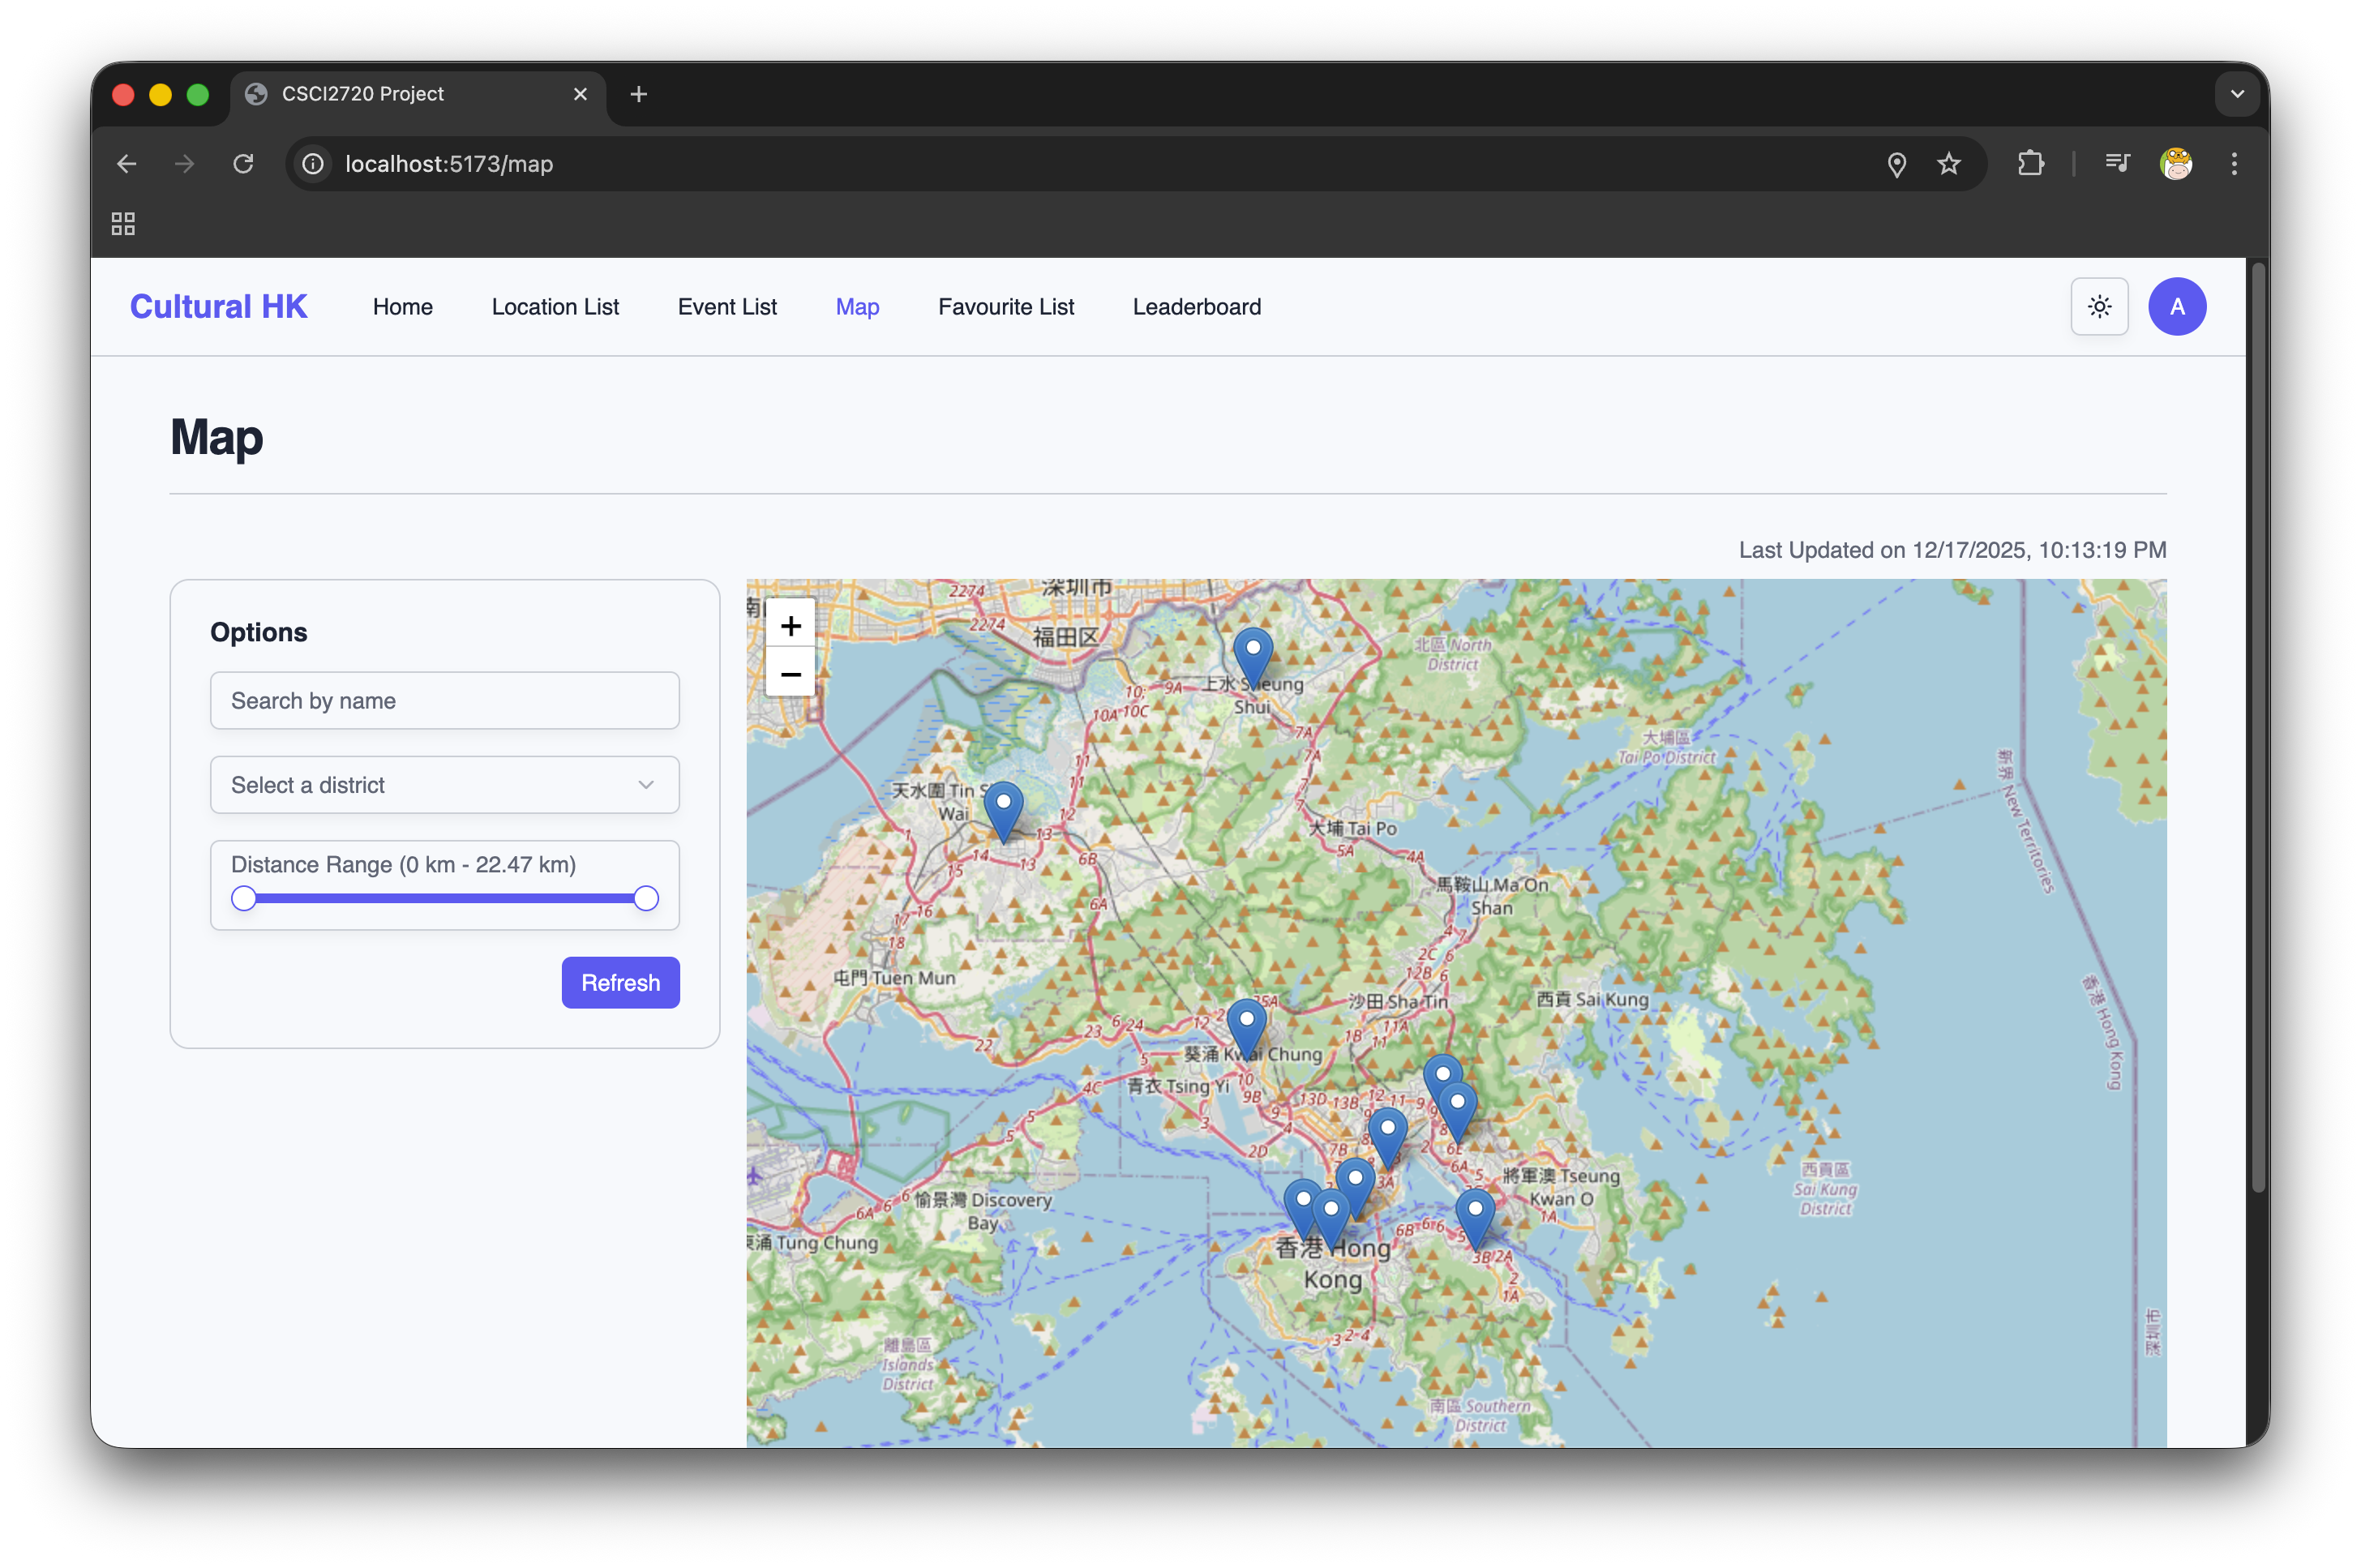
\includegraphics[width=\textwidth]{figures/req2a.png}
        \caption{See all locations on the map}
        \label{subfig:req2a}
    \end{subfigure}
    \begin{subfigure}{.45\textwidth}
        \centering
        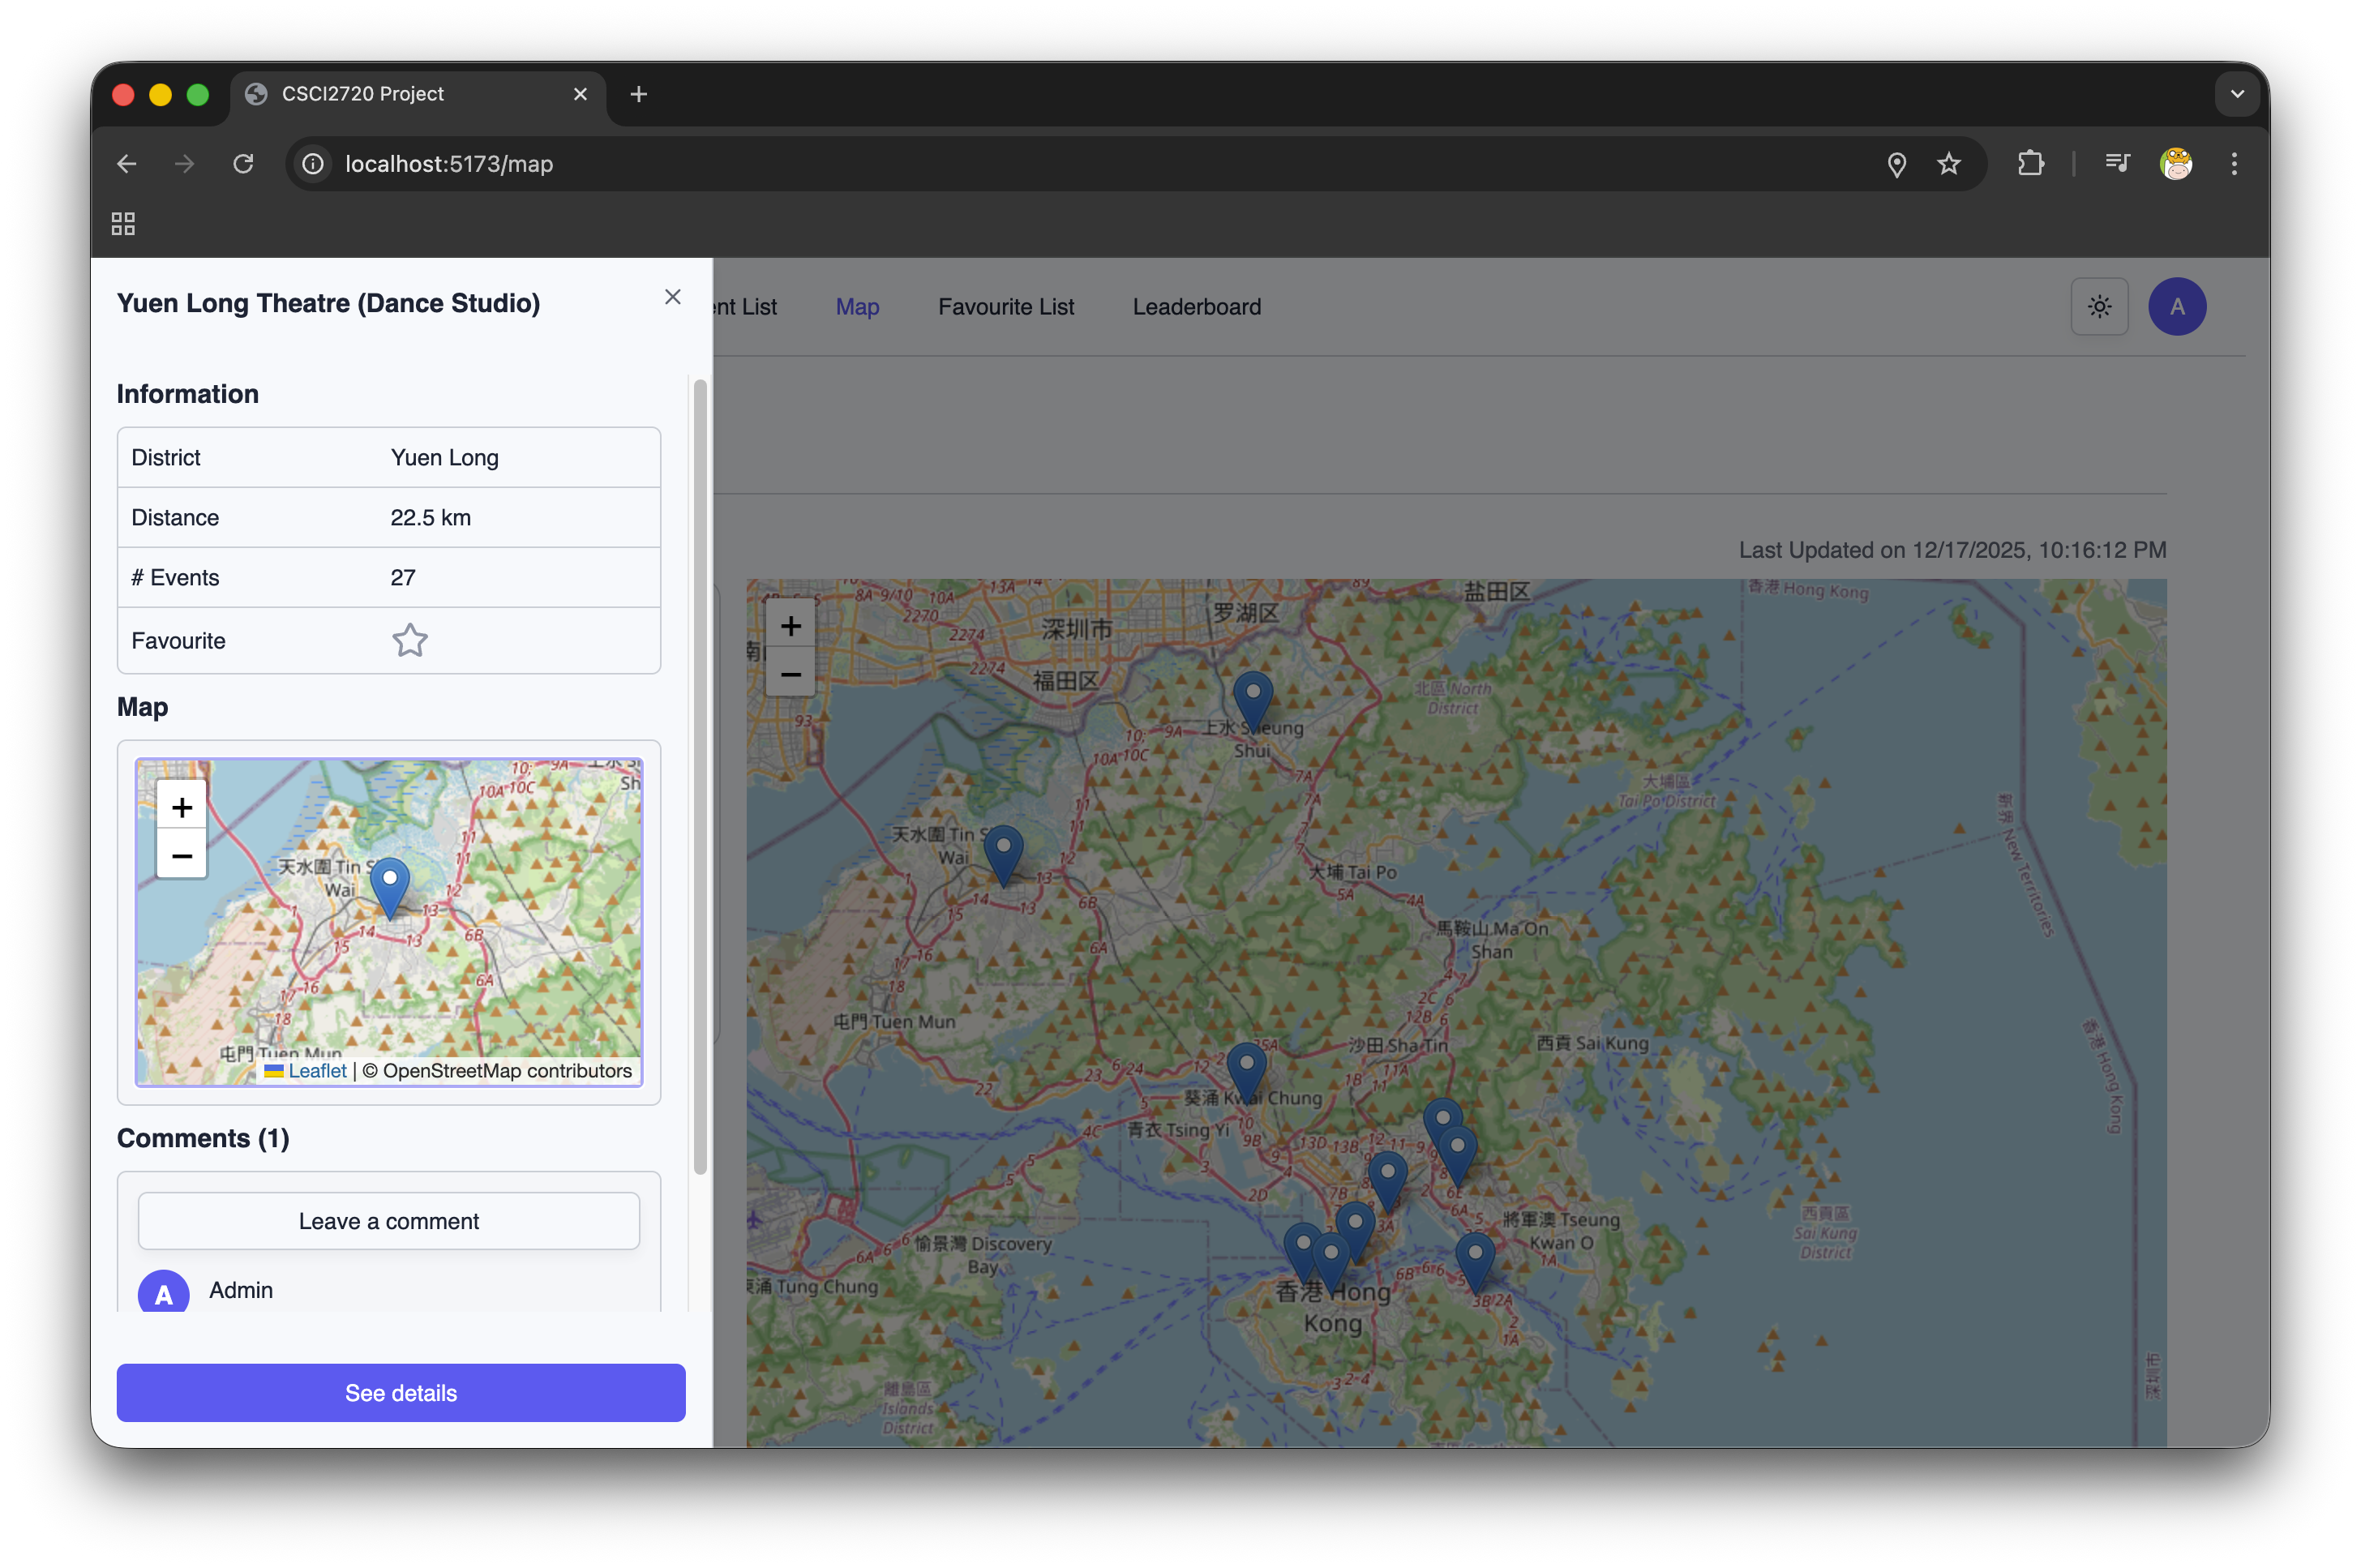
\includegraphics[width=\textwidth]{figures/req2b.png}
        \caption{
            Simply click on a marker to see location details.
        }
        \label{subfig:req2b}
    \end{subfigure}
    \caption{Map}
    \label{fig:map}
\end{figure}

\subsubsection{Requirement 3}
Filter locations by keywords, areas, and distance (e.g., within x km), with dynamic
updates to the location list and map without page refresh.
\begin{figure}[!h]
    \centering
    \begin{subfigure}{0.3\textwidth}
        \centering
        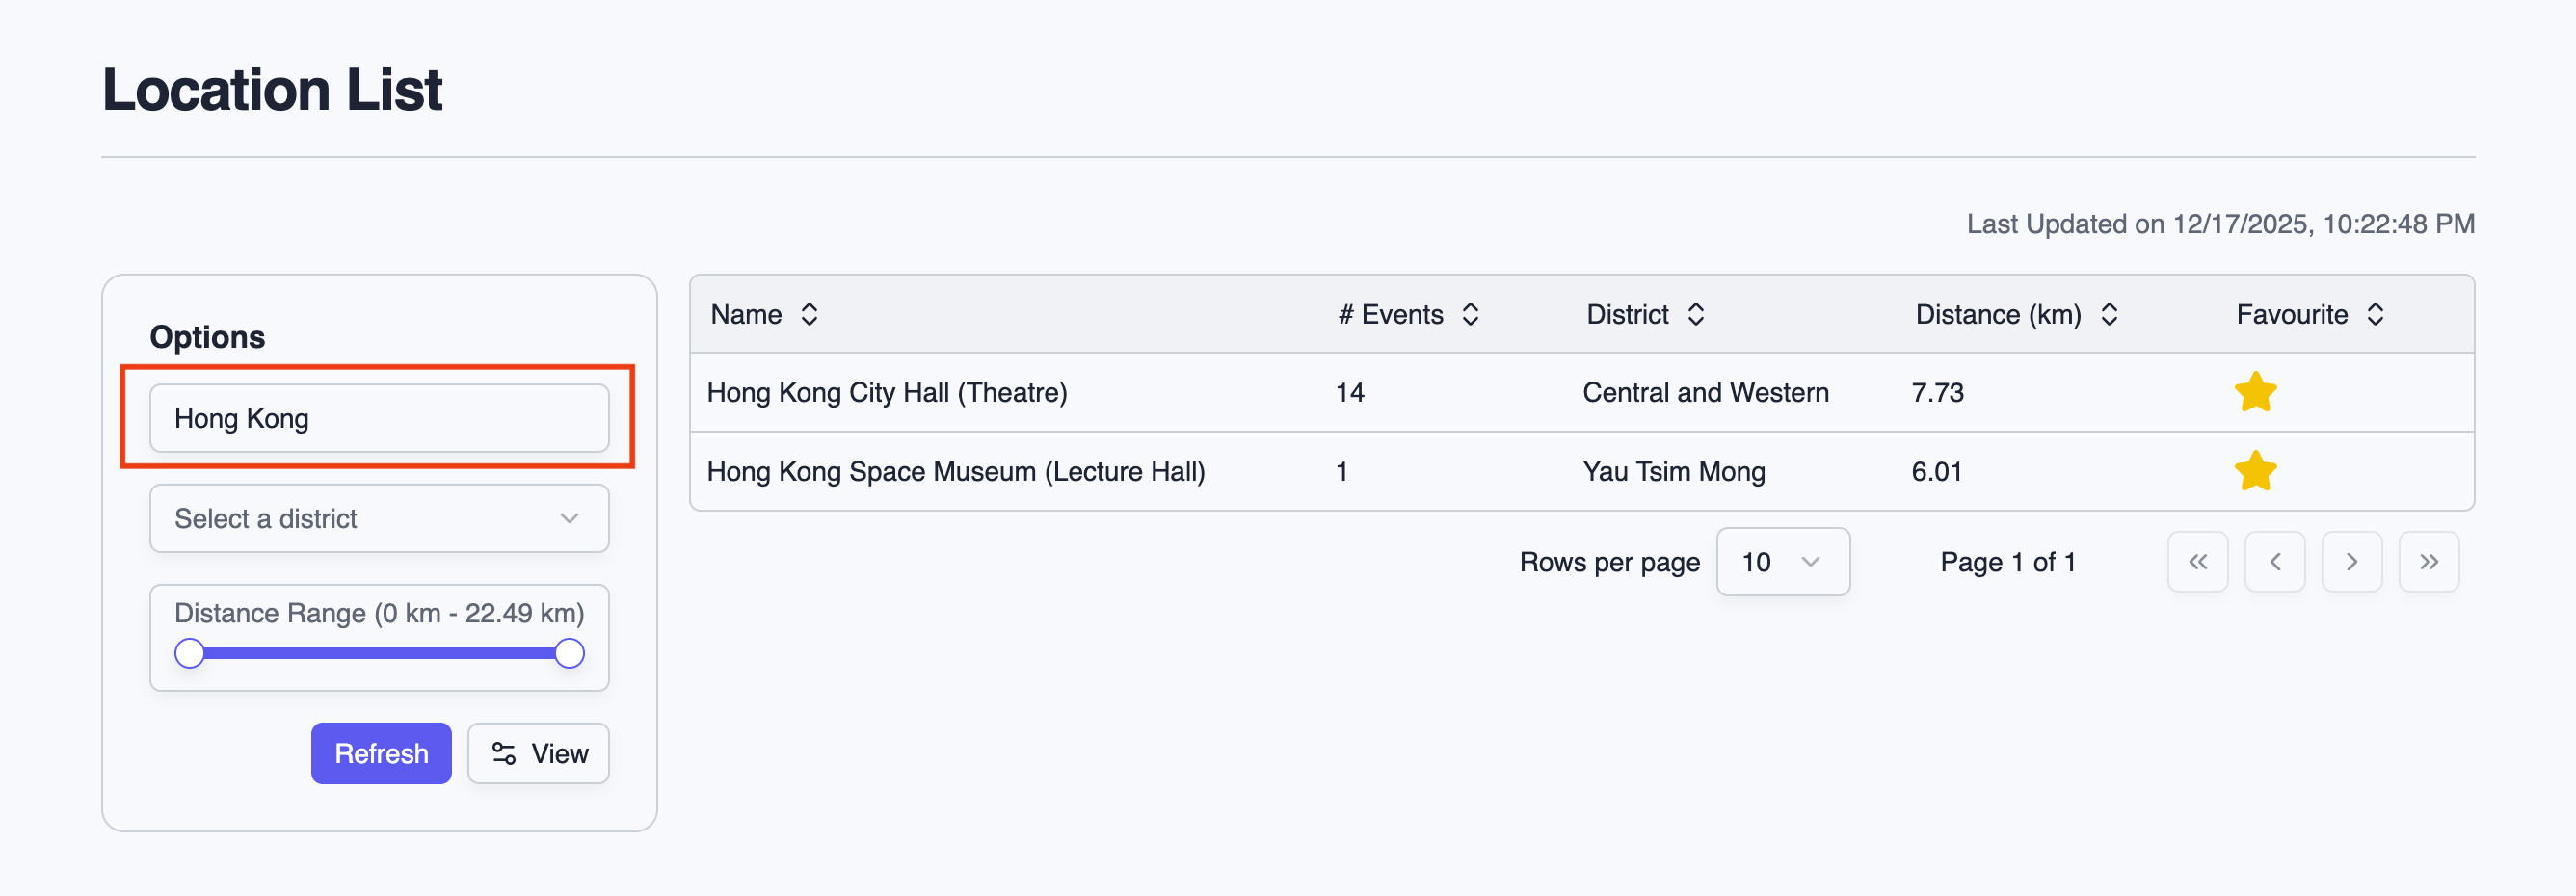
\includegraphics[width=\textwidth]{figures/req3a.png}
        \caption{Filtering with keyword (name)}
        \label{subfig:req3a}
    \end{subfigure}
    \begin{subfigure}{0.3\textwidth}
        \centering
        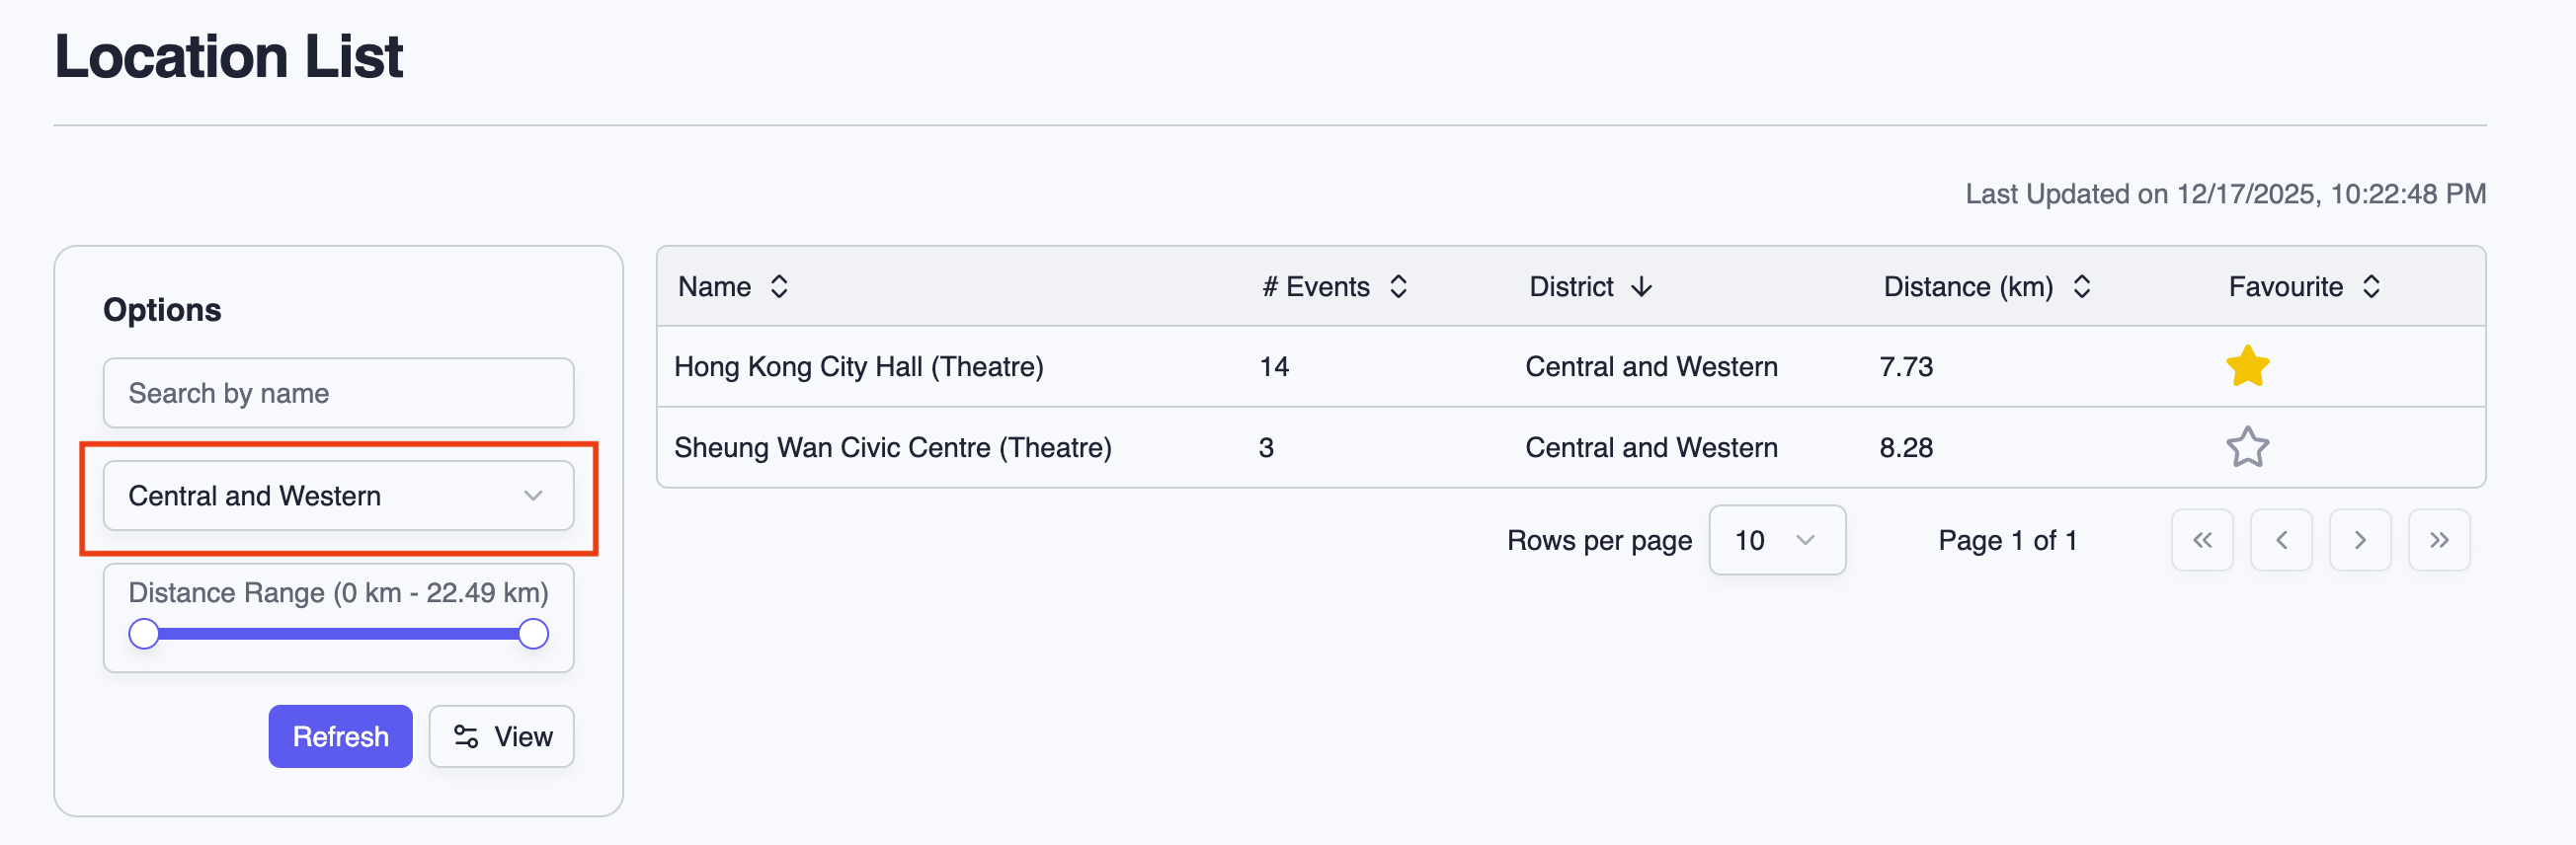
\includegraphics[width=\textwidth]{figures/req3b.png}
        \caption{Filtering by area (district)}
        \label{subfig:req3b}
    \end{subfigure}
    \begin{subfigure}{0.3\textwidth}
        \centering
        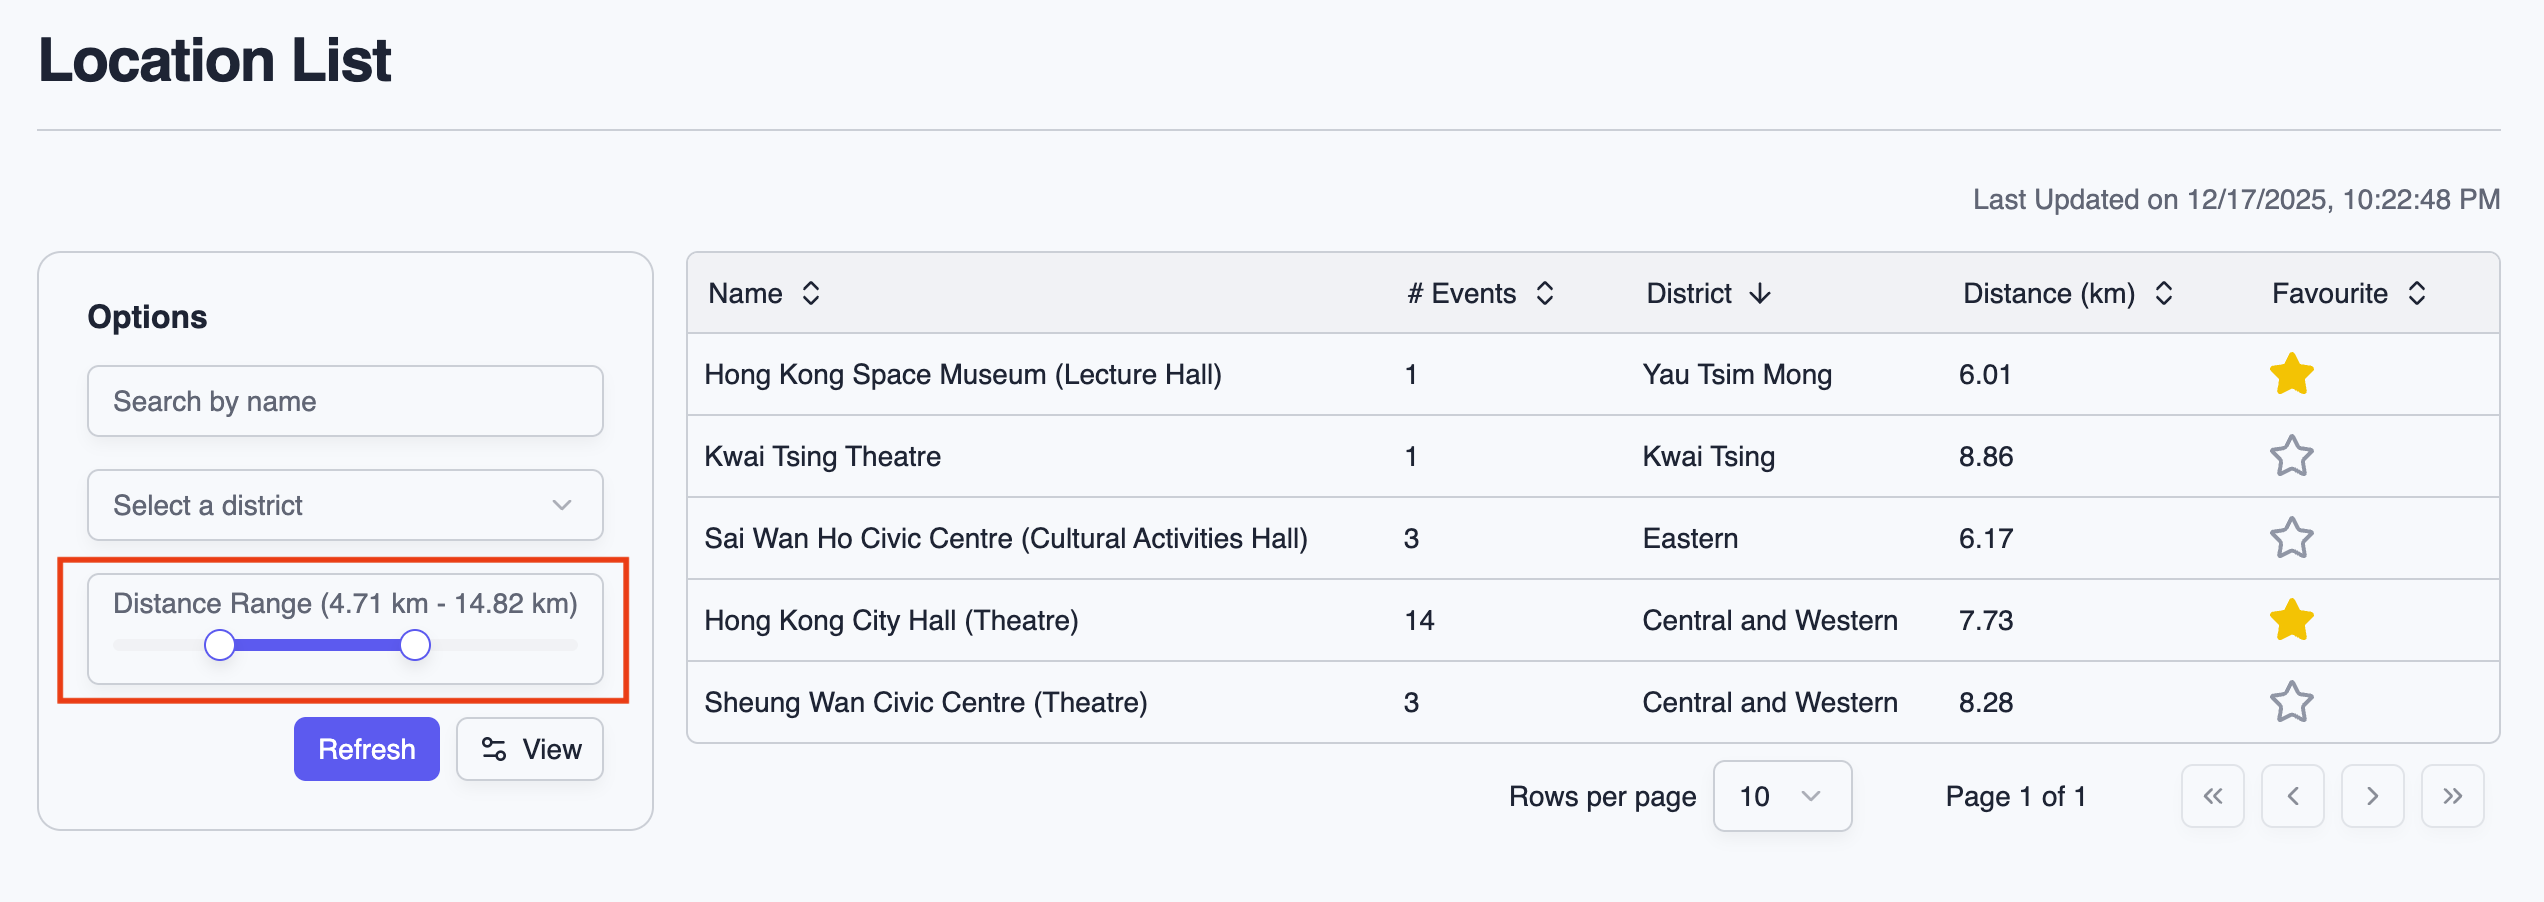
\includegraphics[width=\textwidth]{figures/req3c.png}
        \caption{Filtering by distance}
        \label{subfig:req3c}
    \end{subfigure}
    \caption{Location List filtering}
    \label{fig:location_list_filter}
\end{figure}

\subsubsection{Requirement 4}
\begin{wrapfigure}{r}{0.4\textwidth}
    \centering
    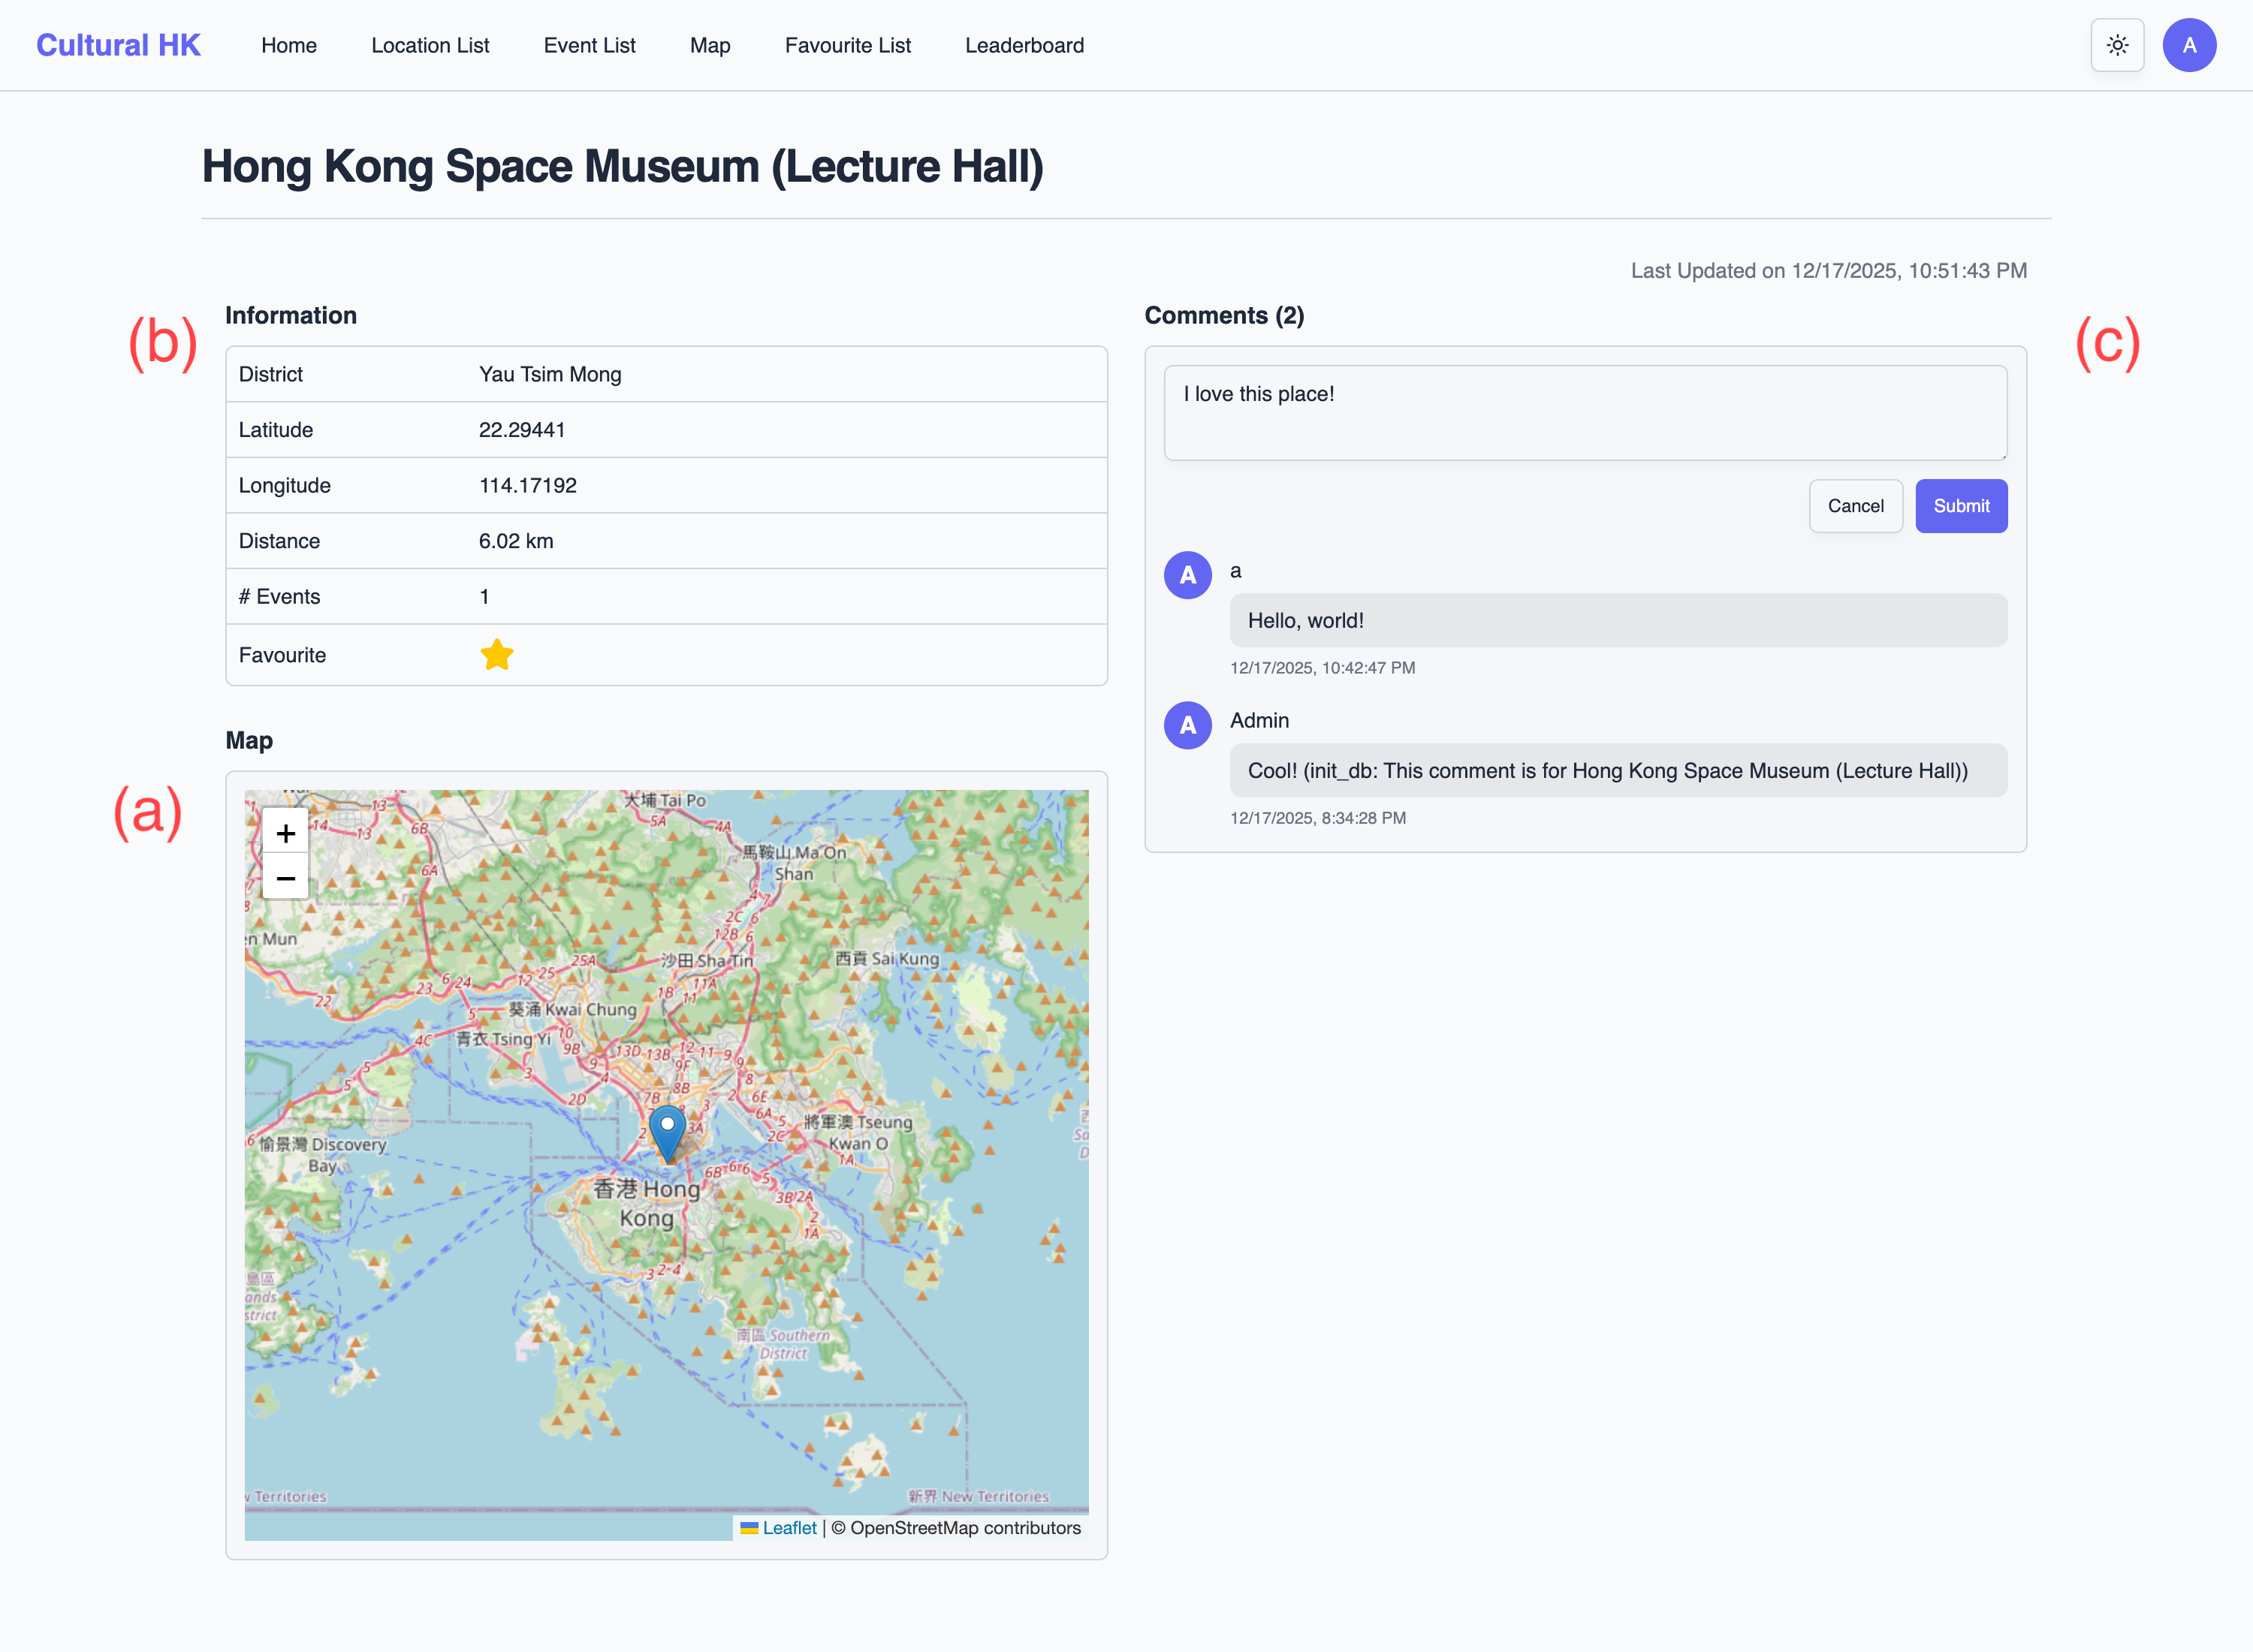
\includegraphics[width=0.3\textwidth]{figures/req4.png}
    \caption{Location detail view}
    \label{fig:req4}
\end{wrapfigure}
A separate view for one single location, containing
\begin{itemize}%[leftmargin=*]
    \item[(a)] A map showing the location.
    \item[(b)] The location details.
    \item[(c)] User comments, where users can add new comments seen by all other users.
\end{itemize}

\newpage
\subsubsection{Requirement 5}
Add location into a list of user's favourite 
locations and see the list in another view.
\begin{figure}[!h]
    \centering
    \begin{subfigure}{.3\textwidth}
        \centering
        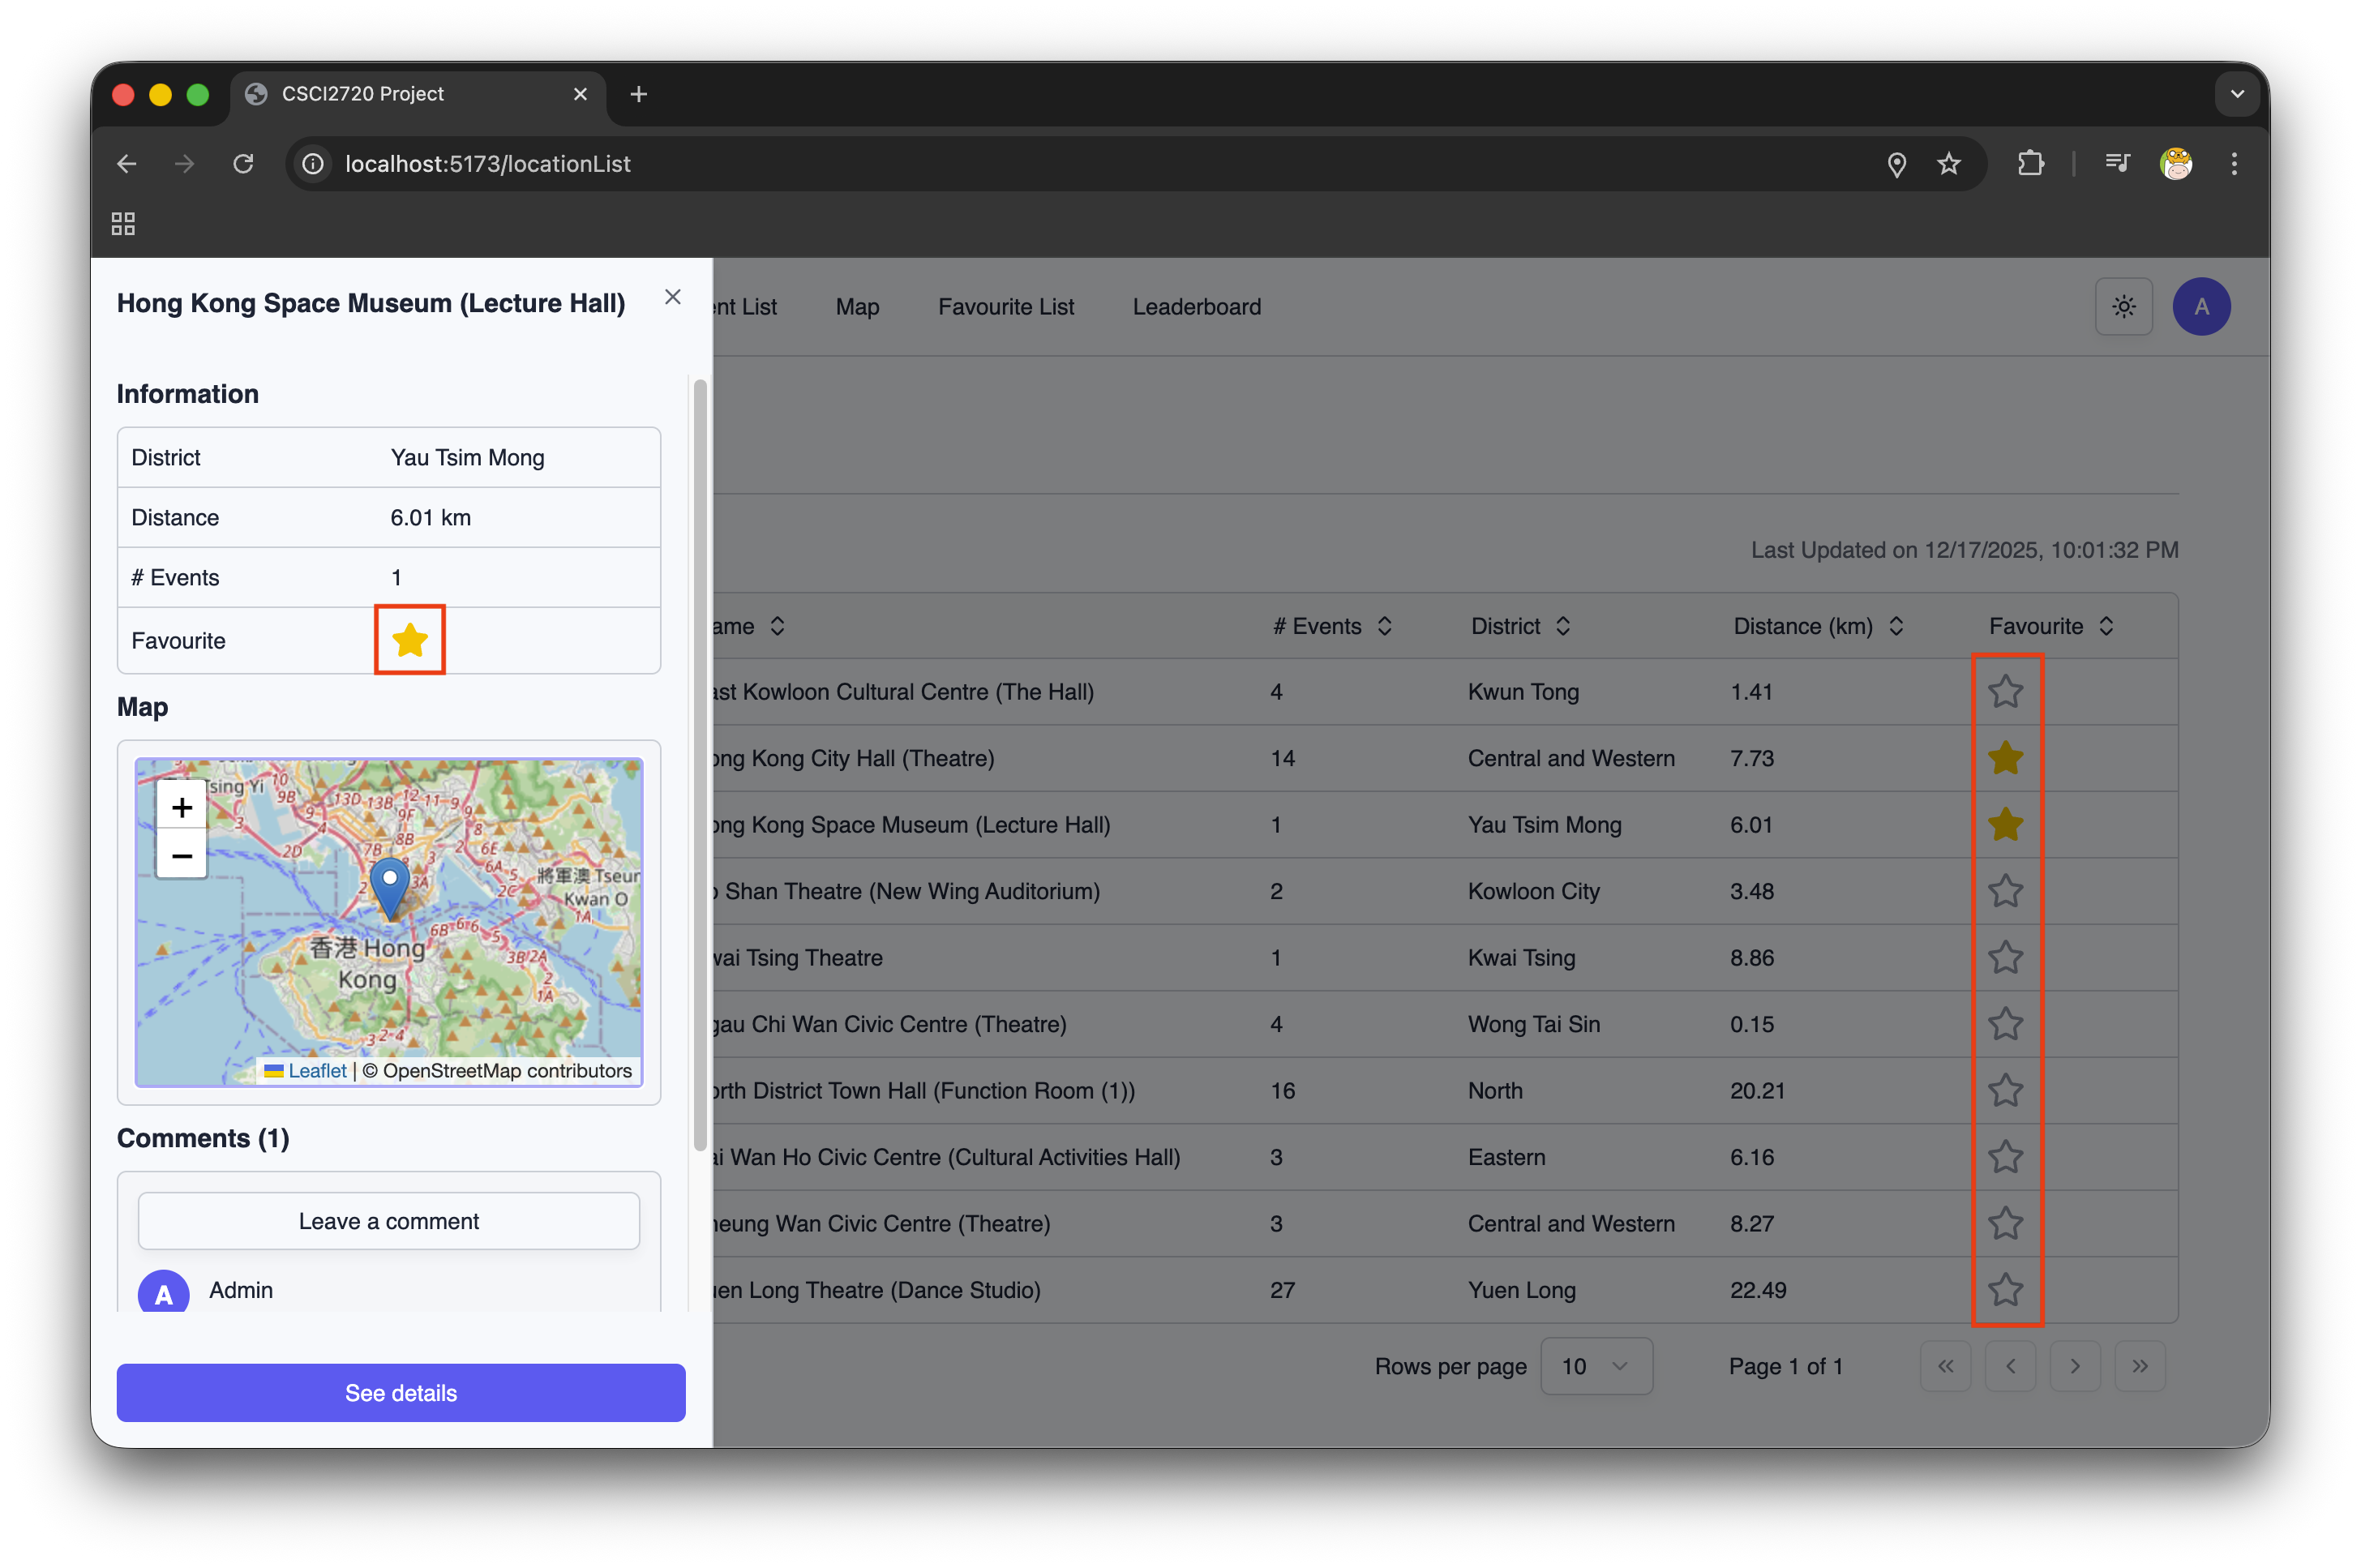
\includegraphics[width=\textwidth]{figures/req5a.png}
        \caption{Click on any stars to toggle favourite.}
        \label{subfig:req5a}
    \end{subfigure}
    \begin{subfigure}{.3\textwidth}
        \centering
        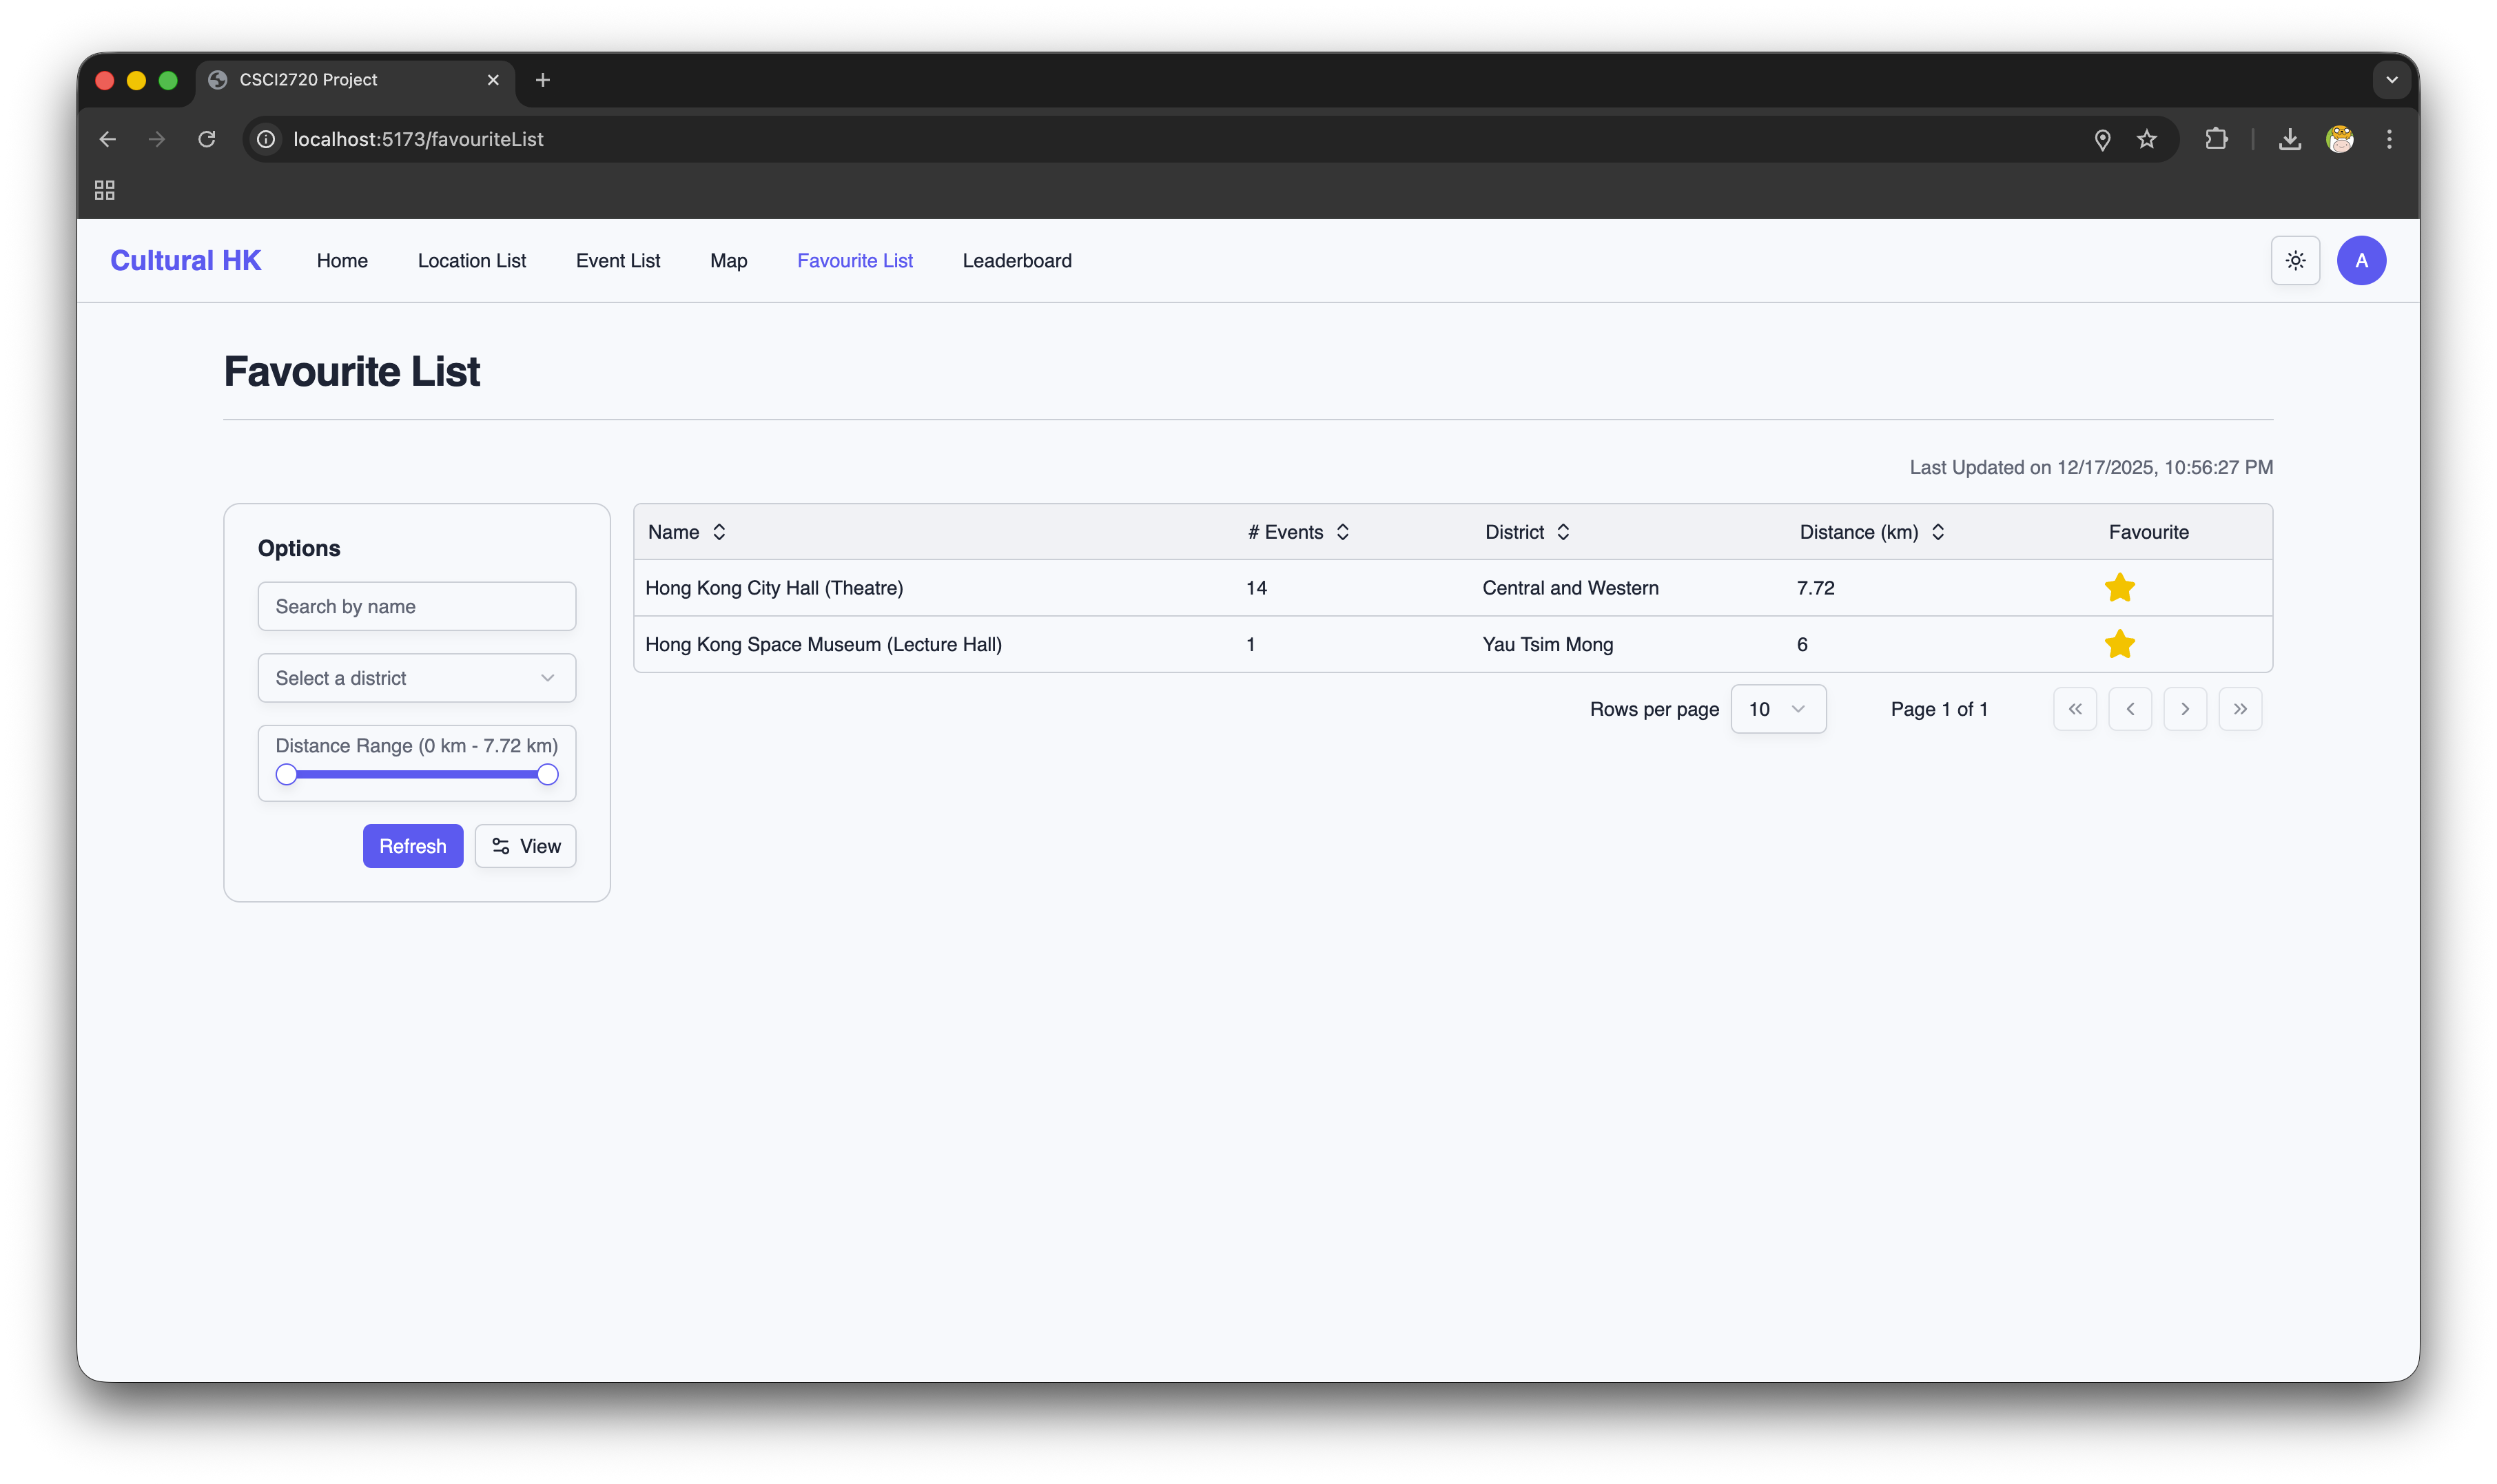
\includegraphics[width=\textwidth]{figures/req5b.png}
        \caption{
            See the list in another view\\\,
        }
        \label{subfig:req5b}
    \end{subfigure}
    \caption{Favourite List}
    \label{fig:favourite_list}
\end{figure}

\subsubsection{Requirement 6}
\label{subsubsec:req6}
See the username in the top-right of screen and be able to log out.
\begin{figure}[h]
    \centering
    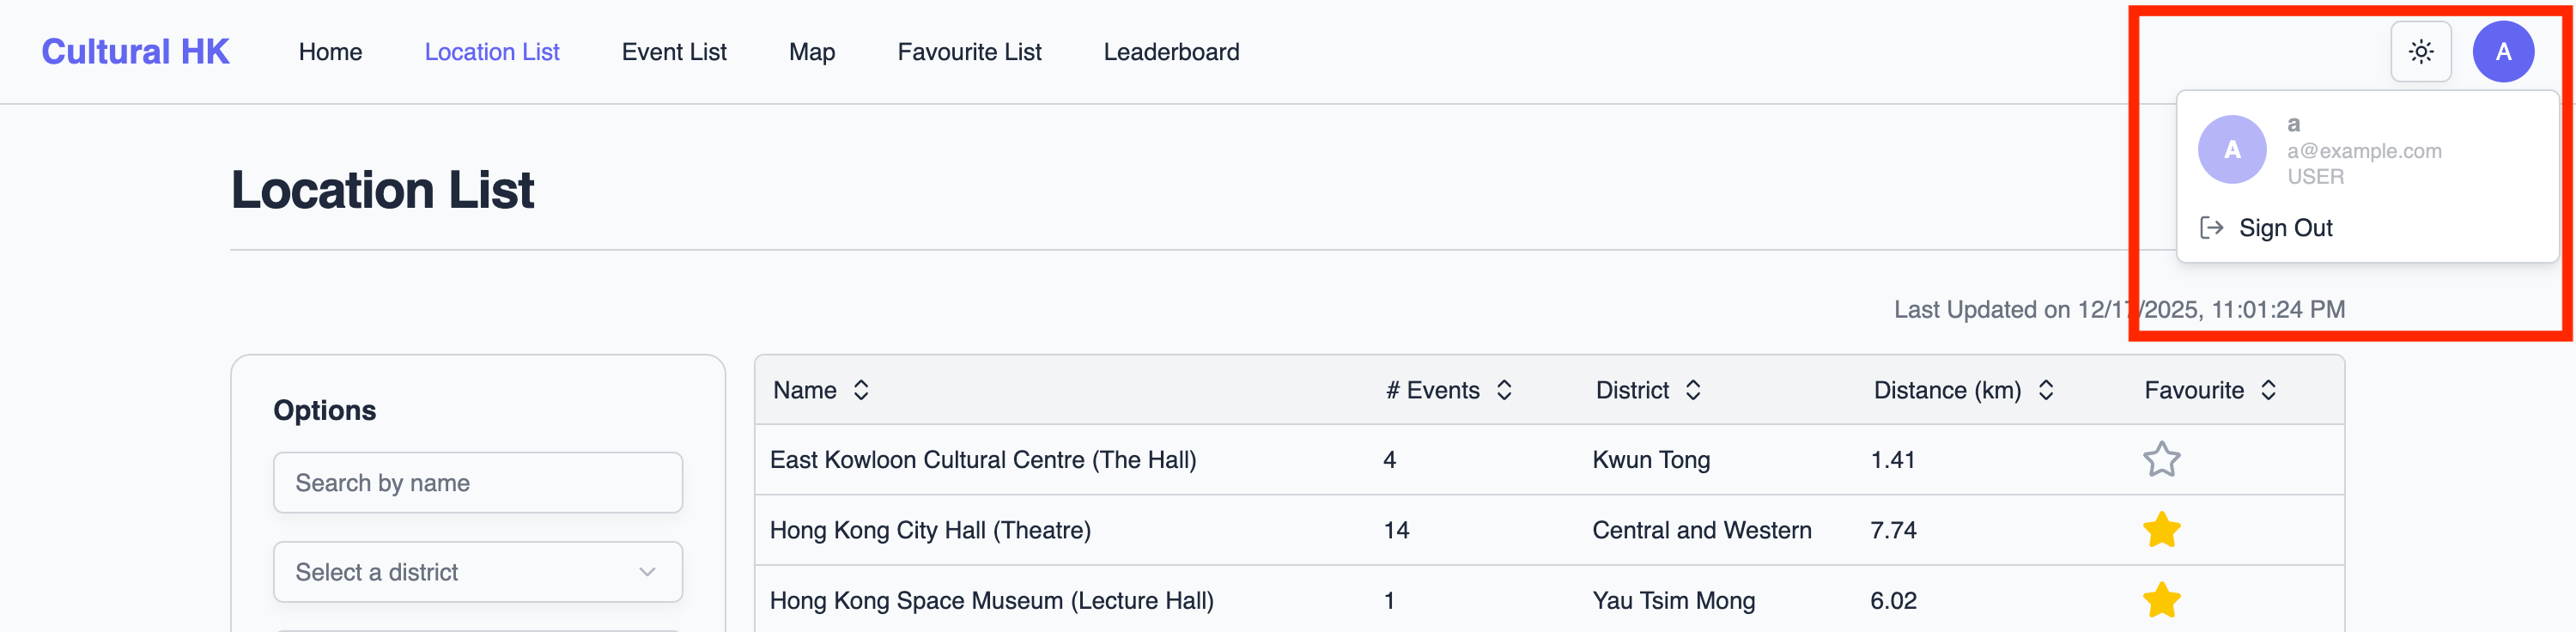
\includegraphics[width=0.5\textwidth]{figures/req6.png}
    \caption{User dropdown menu}
    \label{fig:req6}
\end{figure}